\section*{سوال ۶}

تحلیل روش طراحی ویژگی‌رانه (نسخه سوم) را به دقت مطالعه کنید و تحلیل خود را از این روش براساس موارد زیر بیان کنید.

\section*{مستندات معماری}
شامل تصمیمات، عقلانیت، دیدگاه‌های معماری، راه‌حل‌های جایگزین، بازنمایی و سایر موارد اشاره شده در کتاب.

\section*{نگرانی‌های همه انواع ذی‌نفعان}
شامل کاربر نهایی، مشتری، تیم ایجاد، مدیر پروژه و …

\section*{چگونگی کاربرد مفاهیم، اصول، الگوها و سبک‌های معماری}
بررسی نحوه کاربرد این مفاهیم در روش طراحی ویژگی رانه.

توجه کنید پوشایی و دقت پاسخ شما به عنوان ملاک مهم ارزیابی در این سوال در نظر گرفته می‌شود.

\section*{جواب سوال ۶}

\begin{figure}[H]
	\centering
	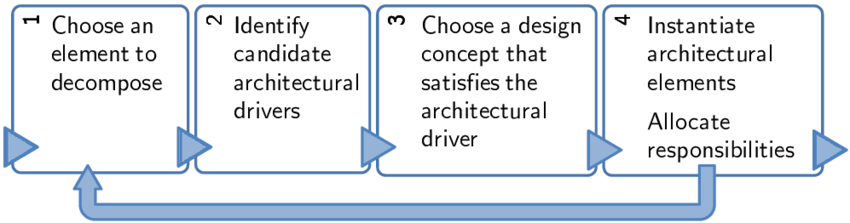
\includegraphics{pic10.png}
	\label{fig:label4}
\end{figure}

روش طراحی ویژگی‌رانه (ADD) یک رویکرد چابک برای توسعه معماری نرم‌افزار است که بر اساس ویژگی‌ها متمرکز است. این روش در سال 2004 توسط دو نفر به نام‌های جف باک و ریچارد هافمن معرفی شد و در سال 2016 نسخه سوم آن منتشر شد.

\subsection*{مستندات معماری}

در روش طراحی ویژگی‌رانه، مستندات معماری به صورت مداوم و در طول فرآیند توسعه ایجاد می‌شود. این مستندات شامل موارد زیر هستند:

\begin{itemize}
	\item دستور کار \lr{(Action Plan)} : 
	این سند شامل جزئیات هر گام از فرآیند طراحی ویژگی‌رانه است. این سند باید شامل موارد زیر باشد:
	
	اهداف هر گام
	
	فعالیت‌های مورد نیاز برای رسیدن به اهداف
	
	زمان‌بندی هر فعالیت
	
	منابع مورد نیاز برای هر فعالیت
	\item استانداردها و الگوها \lr{(Standards and Patterns)} :
	این سند شامل استانداردها و الگوهای مورد استفاده در طراحی معماری است. این سند باید شامل موارد زیر باشد:
	
	استانداردهای فنی، مانند استانداردهای زبان برنامه‌نویسی، استانداردهای پایگاه داده، و استانداردهای امنیت
	
	الگوهای معمارانه، مانند الگوهای سه‌لایه، MVC ، و MVVM
	\item توضیحات معماری \lr{(Architecture Description)} :
	
	این سند شامل توضیحات کامل از معماری نرم‌افزار است. این سند باید شامل موارد زیر باشد:
	
	اجزای نرم‌افزار
	
	روابط بین اجزای نرم‌افزار
	
	ویژگی‌های نرم‌افزار
	
	محدودیت‌های نرم‌افزار
\end{itemize}

این مستندات باید به گونه‌ای تهیه شوند که برای همه ذی‌نفعان قابل فهم باشند.

\subsection*{نگرانی‌های همه انواع ذی‌نفعان}

روش طراحی ویژگی‌رانه بر اهمیت توجه به نگرانی‌های همه انواع ذی‌نفعان تأکید دارد. این ذی‌نفعان شامل موارد زیر هستند:

\begin{itemize}
	\item کاربر نهایی \lr{(End User)} :
	افرادی که نرم‌افزار را استفاده می‌کنند. نگرانی‌های این افراد شامل موارد زیر است:
	
	کارایی نرم‌افزار
	
	سهولت استفاده از نرم‌افزار
	
	قابلیت اطمینان نرم‌افزار
	
	\item مشتری \lr{(Customer)} :
	افرادی که نرم‌افزار را سفارش می‌دهند. نگرانی‌های این افراد شامل موارد زیر است:
	
	هزینه نرم‌افزار
	
	زمان تحویل نرم‌افزار
	
	الزامات قانونی نرم‌افزار
	
	\item تیم ایجاد \lr{(Development Team)} :
	افرادی که نرم‌افزار را توسعه می‌دهند. نگرانی‌های این افراد شامل موارد زیر است:
	پیچیدگی نرم‌افزار
	
	قابلیت نگهداری نرم‌افزار
	
	قابلیت توسعه‌پذیری نرم‌افزار
	
	\item مدیر پروژه \lr{(Project Manager)} :
	افرادی که پروژه توسعه نرم‌افزار را مدیریت می‌کنند. نگرانی‌های این افراد شامل موارد زیر است:
	
	ریسک‌های پروژه
	
	زمان‌بندی پروژه
	
	بودجه پروژه
\end{itemize}

روش طراحی ویژگی‌رانه به ذی‌نفعان کمک می‌کند تا در فرآیند طراحی معماری مشارکت داشته باشند و نگرانی‌های خود را بیان کنند.

\subsection*{چگونگی کاربرد مفاهیم، اصول، الگوها و سبک‌های معماری}

روش طراحی ویژگی‌رانه از مفاهیم، اصول، الگوها و سبک‌های معماری برای ایجاد یک معماری نرم‌افزار کارآمد و پایدار استفاده می‌کند. این مفاهیم، اصول، الگوها و سبک‌ها عبارتند از:

\begin{itemize}
	\item مفاهیم معماری: مانند مفاهیم سیستم‌های باز، سیستم‌های توزیع‌شده و سیستم‌های چند لایه.
	
	\item اصول معماری:
	 مانند اصل انتزاع، اصل تفکیک وظایف و اصل وابستگی ضعیف.
	
	\item الگوهای معماری:
	 مانند الگوهای معمارانه مشترک مانند سه‌لایه، MVC و MVVM .
	 
	 \item سبک‌های معماری: اینها روش‌هایی هستند که بیانگر یک رویکرد کلی در طراحی معماری هستند. سبک‌های معماری مانند معماری میکروسرویس‌ها، معماری مبتنی بر رویداد و معماری سرویس گرا (SOA) تاکید بر اصولی مانند تجزیه و تحلیل، توزیع وزنی کارکردها و تعامل میان سرویس‌های مستقل دارند. این سبک‌ها به معماران کمک می‌کنند تا سیستم‌هایی پیچیده و قابل توسعه را طراحی کنند که بتوانند به خوبی در محیط‌های پیچیده و متغیر پاسخگو باشند.
	 
\end{itemize}
	 
در نهایت، این مفاهیم، اصول، الگوها و سبک‌های معماری به معماران نرم‌افزار این امکان را می‌دهند تا سیستم‌هایی ایجاد کنند که نه تنها به خوبی عمل می‌کنند بلکه قابلیت انعطاف و تطابق با تغییرات آینده را نیز دارند.

\begin{figure}[H]
	\centering
	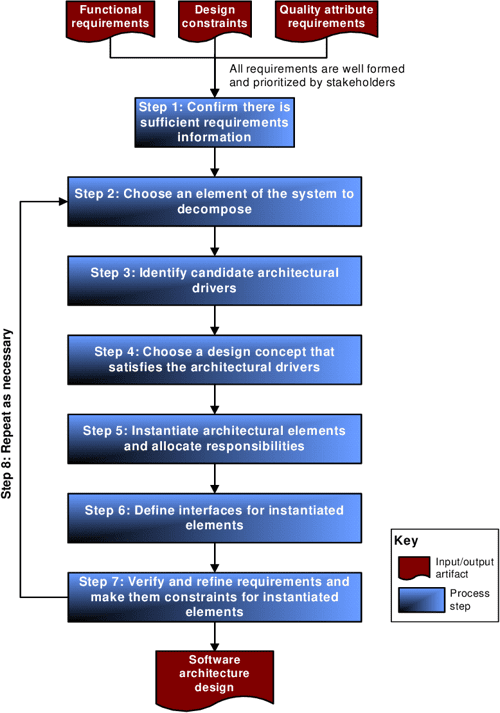
\includegraphics{pic11.png}
	\label{fig:label4}
\end{figure}